\documentclass{standalone}

\usepackage[english]{babel}
\usepackage[utf8x]{inputenc}
\usepackage[T1]{fontenc}
\usepackage{tikz,pgf} %and any other packages or tikzlibraries your picture needs
\usepackage{amsfonts}
\usepackage{amsmath}
\usepackage{physics}
\usepackage{amssymb}
\usepackage{mathtools}
\usetikzlibrary{shapes,arrows,patterns}

\begin{document}

%%%%%%%%%%%%%%%%%%%%%%%%%%%%%%%%%%%%%%%%%%%%%%%%%%%%%%%%%%%%%%%%%%%%%%%%%%%%%%%%
%COPY HERE
%%%%%%%%%%%%%%%%%%%%%%%%%%%%%%%%%%%%%%%%%%%%%%%%%%%%%%%%%%%%%%%%%%%%%%%%%%%%%%%%



\tikzset{every picture/.style={line width=0.75pt}} %set default line width to 0.75pt

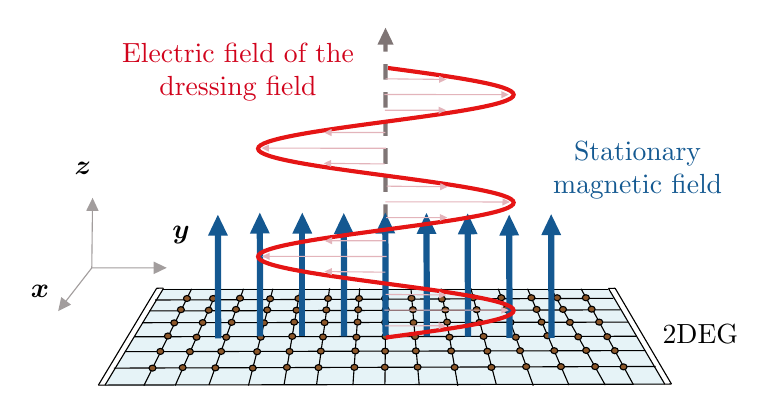
\begin{tikzpicture}[x=0.75pt,y=0.75pt,yscale=-1,xscale=1]
%uncomment if require: \path (0,300); %set diagram left start at 0, and has height of 300

%Straight Lines [id:da5726274877822322]
\draw [color={rgb, 255:red, 127; green, 117; blue, 117 }  ,draw opacity=1 ][line width=1.5]  [dash pattern={on 5.63pt off 4.5pt}]  (339.92,108.44) -- (339.87,253.18) ;
\draw [shift={(339.92,104.44)}, rotate = 90.02] [fill={rgb, 255:red, 127; green, 117; blue, 117 }  ,fill opacity=1 ][line width=0.08]  [draw opacity=0] (8.13,-3.9) -- (0,0) -- (8.13,3.9) -- cycle    ;
%Straight Lines [id:da29209126760206683]
\draw [color={rgb, 255:red, 162; green, 157; blue, 157 }  ,draw opacity=1 ]   (198.39,220.13) -- (231.49,220.09) ;
\draw [shift={(234.49,220.09)}, rotate = 539.9300000000001] [fill={rgb, 255:red, 162; green, 157; blue, 157 }  ,fill opacity=1 ][line width=0.08]  [draw opacity=0] (6.25,-3) -- (0,0) -- (6.25,3) -- cycle    ;
%Straight Lines [id:da6165306544380005]
\draw [color={rgb, 255:red, 162; green, 157; blue, 157 }  ,draw opacity=1 ]   (198.39,220.13) -- (184.04,238.58) ;
\draw [shift={(182.2,240.94)}, rotate = 307.89] [fill={rgb, 255:red, 162; green, 157; blue, 157 }  ,fill opacity=1 ][line width=0.08]  [draw opacity=0] (6.25,-3) -- (0,0) -- (6.25,3) -- cycle    ;
%Straight Lines [id:da7391727465011027]
\draw [color={rgb, 255:red, 162; green, 157; blue, 157 }  ,draw opacity=1 ]   (198.39,220.13) -- (198.74,189.37) ;
\draw [shift={(198.77,186.37)}, rotate = 450.64] [fill={rgb, 255:red, 162; green, 157; blue, 157 }  ,fill opacity=1 ][line width=0.08]  [draw opacity=0] (6.25,-3) -- (0,0) -- (6.25,3) -- cycle    ;


%Shape: Parallelogram [id:dp41534268368743876]
\draw  [color={rgb, 255:red, 230; green, 243; blue, 247 }  ,draw opacity=1 ][fill={rgb, 255:red, 230; green, 243; blue, 247 }  ,fill opacity=1 ] (233.03,230.41) -- (281.59,230.41) -- (253.7,276.83) -- (205.14,276.83) -- cycle ;
%Shape: Trapezoid [id:dp7788778266108187]
\draw  [color={rgb, 255:red, 230; green, 243; blue, 247 }  ,draw opacity=1 ][fill={rgb, 255:red, 230; green, 243; blue, 247 }  ,fill opacity=1 ] (248.48,276.13) -- (248.97,230.43) -- (447.07,230.43) -- (473.99,276.13) -- cycle ;
%Straight Lines [id:da5683506349044234]
\draw [fill={rgb, 255:red, 139; green, 87; blue, 42 }  ,fill opacity=1 ]   (204.78,276.57) -- (474.45,276.13) ;
%Straight Lines [id:da36516960272690935]
\draw [fill={rgb, 255:red, 139; green, 87; blue, 42 }  ,fill opacity=1 ]   (232.53,230.41) -- (446.93,230.41) ;
%Straight Lines [id:da218377945892541]
\draw [fill={rgb, 255:red, 139; green, 87; blue, 42 }  ,fill opacity=1 ]   (232.93,230.01) -- (204.78,276.57) ;
%Straight Lines [id:da5092960488933624]
\draw [fill={rgb, 255:red, 139; green, 87; blue, 42 }  ,fill opacity=1 ]   (447.33,230.01) -- (474.45,276.13) ;
%Straight Lines [id:da11082740586756445]
\draw [fill={rgb, 255:red, 139; green, 87; blue, 42 }  ,fill opacity=1 ]   (340.13,230.01) -- (339.62,276.35) ;
%Straight Lines [id:da2154900622918119]
\draw [fill={rgb, 255:red, 139; green, 87; blue, 42 }  ,fill opacity=1 ]   (327.45,229.97) -- (324.21,276.57) ;
%Straight Lines [id:da2109844821797362]
\draw [fill={rgb, 255:red, 139; green, 87; blue, 42 }  ,fill opacity=1 ]   (312.94,229.97) -- (306.71,276.31) ;
%Straight Lines [id:da14123000440106437]
\draw [fill={rgb, 255:red, 139; green, 87; blue, 42 }  ,fill opacity=1 ]   (298.83,229.92) -- (291.06,276.31) ;
%Straight Lines [id:da6719175270526567]
\draw [fill={rgb, 255:red, 139; green, 87; blue, 42 }  ,fill opacity=1 ]   (285.63,230.19) -- (273.86,276.83) ;
%Straight Lines [id:da7130190425909961]
\draw [fill={rgb, 255:red, 139; green, 87; blue, 42 }  ,fill opacity=1 ]   (271.49,230.21) -- (254.83,276.57) ;
%Straight Lines [id:da02923644984301399]
\draw [fill={rgb, 255:red, 139; green, 87; blue, 42 }  ,fill opacity=1 ]   (259.23,230.19) -- (238.56,276.83) ;
%Straight Lines [id:da44595644058071016]
\draw [fill={rgb, 255:red, 139; green, 87; blue, 42 }  ,fill opacity=1 ]   (246.51,230.21) -- (223.51,276.83) ;
%Straight Lines [id:da03090530016819959]
\draw [fill={rgb, 255:red, 139; green, 87; blue, 42 }  ,fill opacity=1 ]   (352.15,229.92) -- (356.14,276.57) ;
%Straight Lines [id:da0075347964569616455]
\draw [fill={rgb, 255:red, 139; green, 87; blue, 42 }  ,fill opacity=1 ]   (366.71,230.09) -- (374.75,276.93) ;
%Straight Lines [id:da9231431383372868]
\draw [fill={rgb, 255:red, 139; green, 87; blue, 42 }  ,fill opacity=1 ]   (381.01,229.92) -- (393.29,276.31) ;
%Straight Lines [id:da5734645298908272]
\draw [fill={rgb, 255:red, 139; green, 87; blue, 42 }  ,fill opacity=1 ]   (394.21,230.19) -- (411.1,276.83) ;
%Straight Lines [id:da18417258051367602]
\draw [fill={rgb, 255:red, 139; green, 87; blue, 42 }  ,fill opacity=1 ]   (408.34,230.19) -- (428.29,276.57) ;
%Straight Lines [id:da7766509629904832]
\draw [fill={rgb, 255:red, 139; green, 87; blue, 42 }  ,fill opacity=1 ]   (419.7,230.09) -- (445.79,276.57) ;
%Straight Lines [id:da5541997421952078]
\draw [fill={rgb, 255:red, 139; green, 87; blue, 42 }  ,fill opacity=1 ]   (434.13,230.19) -- (459.3,276.31) ;
%Straight Lines [id:da8163512478619217]
\draw [fill={rgb, 255:red, 139; green, 87; blue, 42 }  ,fill opacity=1 ]   (209.08,268.4) -- (470.05,267.61) ;
%Straight Lines [id:da6866382299263494]
\draw [fill={rgb, 255:red, 139; green, 87; blue, 42 }  ,fill opacity=1 ]   (214.3,260.49) -- (465.14,259.97) ;
%Straight Lines [id:da10951428264342855]
\draw [fill={rgb, 255:red, 139; green, 87; blue, 42 }  ,fill opacity=1 ]   (218.86,253.29) -- (460.89,253.07) ;
%Straight Lines [id:da16627986420586138]
\draw [fill={rgb, 255:red, 139; green, 87; blue, 42 }  ,fill opacity=1 ]   (222.59,246.53) -- (456.85,246.26) ;
%Straight Lines [id:da1104010543118994]
\draw [fill={rgb, 255:red, 139; green, 87; blue, 42 }  ,fill opacity=1 ]   (226.18,240.86) -- (453.07,240.34) ;
%Straight Lines [id:da46889737940339105]
\draw [fill={rgb, 255:red, 139; green, 87; blue, 42 }  ,fill opacity=1 ]   (228.95,235.59) -- (449.69,234.8) ;
%Shape: Ellipse [id:dp7799971866902644]
\draw  [fill={rgb, 255:red, 139; green, 87; blue, 42 }  ,fill opacity=1 ] (225.97,268.4) .. controls (225.97,267.6) and (226.73,266.95) .. (227.66,266.95) .. controls (228.59,266.95) and (229.35,267.6) .. (229.35,268.4) .. controls (229.35,269.2) and (228.59,269.85) .. (227.66,269.85) .. controls (226.73,269.85) and (225.97,269.2) .. (225.97,268.4) -- cycle ;
%Shape: Ellipse [id:dp33000551716975157]
\draw  [fill={rgb, 255:red, 139; green, 87; blue, 42 }  ,fill opacity=1 ] (229.74,260.37) .. controls (229.74,259.57) and (230.49,258.92) .. (231.43,258.92) .. controls (232.36,258.92) and (233.11,259.57) .. (233.11,260.37) .. controls (233.11,261.17) and (232.36,261.82) .. (231.43,261.82) .. controls (230.49,261.82) and (229.74,261.17) .. (229.74,260.37) -- cycle ;
%Shape: Ellipse [id:dp06335085811101071]
\draw  [fill={rgb, 255:red, 139; green, 87; blue, 42 }  ,fill opacity=1 ] (233.37,252.95) .. controls (233.37,252.15) and (234.12,251.5) .. (235.05,251.5) .. controls (235.99,251.5) and (236.74,252.15) .. (236.74,252.95) .. controls (236.74,253.75) and (235.99,254.4) .. (235.05,254.4) .. controls (234.12,254.4) and (233.37,253.75) .. (233.37,252.95) -- cycle ;
%Shape: Ellipse [id:dp5515387996519605]
\draw  [fill={rgb, 255:red, 139; green, 87; blue, 42 }  ,fill opacity=1 ] (236.44,246.6) .. controls (236.44,245.8) and (237.19,245.15) .. (238.12,245.15) .. controls (239.06,245.15) and (239.81,245.8) .. (239.81,246.6) .. controls (239.81,247.4) and (239.06,248.05) .. (238.12,248.05) .. controls (237.19,248.05) and (236.44,247.4) .. (236.44,246.6) -- cycle ;
%Shape: Ellipse [id:dp9613949559203752]
\draw  [fill={rgb, 255:red, 139; green, 87; blue, 42 }  ,fill opacity=1 ] (239.65,240.25) .. controls (239.65,239.45) and (240.4,238.8) .. (241.33,238.8) .. controls (242.27,238.8) and (243.02,239.45) .. (243.02,240.25) .. controls (243.02,241.05) and (242.27,241.7) .. (241.33,241.7) .. controls (240.4,241.7) and (239.65,241.05) .. (239.65,240.25) -- cycle ;
%Shape: Ellipse [id:dp5595749562711418]
\draw  [fill={rgb, 255:red, 139; green, 87; blue, 42 }  ,fill opacity=1 ] (242.58,234.86) .. controls (242.58,234.06) and (243.33,233.41) .. (244.26,233.41) .. controls (245.2,233.41) and (245.95,234.06) .. (245.95,234.86) .. controls (245.95,235.66) and (245.2,236.31) .. (244.26,236.31) .. controls (243.33,236.31) and (242.58,235.66) .. (242.58,234.86) -- cycle ;
%Shape: Ellipse [id:dp9494831013959741]
\draw  [fill={rgb, 255:red, 139; green, 87; blue, 42 }  ,fill opacity=1 ] (240.48,268.16) .. controls (240.48,267.36) and (241.24,266.71) .. (242.17,266.71) .. controls (243.1,266.71) and (243.86,267.36) .. (243.86,268.16) .. controls (243.86,268.96) and (243.1,269.61) .. (242.17,269.61) .. controls (241.24,269.61) and (240.48,268.96) .. (240.48,268.16) -- cycle ;
%Shape: Ellipse [id:dp9210781564959785]
\draw  [fill={rgb, 255:red, 139; green, 87; blue, 42 }  ,fill opacity=1 ] (243.97,260.49) .. controls (243.97,259.69) and (244.73,259.04) .. (245.66,259.04) .. controls (246.59,259.04) and (247.35,259.69) .. (247.35,260.49) .. controls (247.35,261.29) and (246.59,261.94) .. (245.66,261.94) .. controls (244.73,261.94) and (243.97,261.29) .. (243.97,260.49) -- cycle ;
%Shape: Ellipse [id:dp4310038641794769]
\draw  [fill={rgb, 255:red, 139; green, 87; blue, 42 }  ,fill opacity=1 ] (247.2,253.51) .. controls (247.2,252.71) and (247.96,252.06) .. (248.89,252.06) .. controls (249.83,252.06) and (250.58,252.71) .. (250.58,253.51) .. controls (250.58,254.31) and (249.83,254.96) .. (248.89,254.96) .. controls (247.96,254.96) and (247.2,254.31) .. (247.2,253.51) -- cycle ;
%Shape: Ellipse [id:dp03456062696425044]
\draw  [fill={rgb, 255:red, 139; green, 87; blue, 42 }  ,fill opacity=1 ] (250.11,246.48) .. controls (250.11,245.68) and (250.87,245.03) .. (251.8,245.03) .. controls (252.73,245.03) and (253.49,245.68) .. (253.49,246.48) .. controls (253.49,247.28) and (252.73,247.93) .. (251.8,247.93) .. controls (250.87,247.93) and (250.11,247.28) .. (250.11,246.48) -- cycle ;
%Shape: Ellipse [id:dp3303046459338419]
\draw  [fill={rgb, 255:red, 139; green, 87; blue, 42 }  ,fill opacity=1 ] (253.04,240.49) .. controls (253.04,239.69) and (253.8,239.04) .. (254.73,239.04) .. controls (255.66,239.04) and (256.42,239.69) .. (256.42,240.49) .. controls (256.42,241.29) and (255.66,241.94) .. (254.73,241.94) .. controls (253.8,241.94) and (253.04,241.29) .. (253.04,240.49) -- cycle ;
%Shape: Ellipse [id:dp011240288016139521]
\draw  [fill={rgb, 255:red, 139; green, 87; blue, 42 }  ,fill opacity=1 ] (255.14,234.86) .. controls (255.14,234.06) and (255.89,233.41) .. (256.82,233.41) .. controls (257.76,233.41) and (258.51,234.06) .. (258.51,234.86) .. controls (258.51,235.66) and (257.76,236.31) .. (256.82,236.31) .. controls (255.89,236.31) and (255.14,235.66) .. (255.14,234.86) -- cycle ;
%Shape: Ellipse [id:dp6272548395164819]
\draw  [fill={rgb, 255:red, 139; green, 87; blue, 42 }  ,fill opacity=1 ] (256.25,268.28) .. controls (256.25,267.48) and (257.01,266.83) .. (257.94,266.83) .. controls (258.87,266.83) and (259.63,267.48) .. (259.63,268.28) .. controls (259.63,269.08) and (258.87,269.73) .. (257.94,269.73) .. controls (257.01,269.73) and (256.25,269.08) .. (256.25,268.28) -- cycle ;
%Shape: Ellipse [id:dp02366538554974107]
\draw  [fill={rgb, 255:red, 139; green, 87; blue, 42 }  ,fill opacity=1 ] (259.04,260.37) .. controls (259.04,259.57) and (259.8,258.92) .. (260.73,258.92) .. controls (261.66,258.92) and (262.42,259.57) .. (262.42,260.37) .. controls (262.42,261.17) and (261.66,261.82) .. (260.73,261.82) .. controls (259.8,261.82) and (259.04,261.17) .. (259.04,260.37) -- cycle ;
%Shape: Ellipse [id:dp3969356729665663]
\draw  [fill={rgb, 255:red, 139; green, 87; blue, 42 }  ,fill opacity=1 ] (261.48,253.51) .. controls (261.48,252.71) and (262.24,252.06) .. (263.17,252.06) .. controls (264.1,252.06) and (264.86,252.71) .. (264.86,253.51) .. controls (264.86,254.31) and (264.1,254.96) .. (263.17,254.96) .. controls (262.24,254.96) and (261.48,254.31) .. (261.48,253.51) -- cycle ;
%Shape: Ellipse [id:dp6305092289007959]
\draw  [fill={rgb, 255:red, 139; green, 87; blue, 42 }  ,fill opacity=1 ] (264.07,246.36) .. controls (264.07,245.56) and (264.82,244.91) .. (265.76,244.91) .. controls (266.69,244.91) and (267.44,245.56) .. (267.44,246.36) .. controls (267.44,247.16) and (266.69,247.81) .. (265.76,247.81) .. controls (264.82,247.81) and (264.07,247.16) .. (264.07,246.36) -- cycle ;
%Shape: Ellipse [id:dp45941754496129183]
\draw  [fill={rgb, 255:red, 139; green, 87; blue, 42 }  ,fill opacity=1 ] (266.16,240.13) .. controls (266.16,239.33) and (266.92,238.68) .. (267.85,238.68) .. controls (268.78,238.68) and (269.54,239.33) .. (269.54,240.13) .. controls (269.54,240.93) and (268.78,241.58) .. (267.85,241.58) .. controls (266.92,241.58) and (266.16,240.93) .. (266.16,240.13) -- cycle ;
%Shape: Ellipse [id:dp4326662692295993]
\draw  [fill={rgb, 255:red, 139; green, 87; blue, 42 }  ,fill opacity=1 ] (268.11,234.74) .. controls (268.11,233.94) and (268.87,233.29) .. (269.8,233.29) .. controls (270.74,233.29) and (271.49,233.94) .. (271.49,234.74) .. controls (271.49,235.54) and (270.74,236.19) .. (269.8,236.19) .. controls (268.87,236.19) and (268.11,235.54) .. (268.11,234.74) -- cycle ;
%Shape: Ellipse [id:dp5418698275036782]
\draw  [fill={rgb, 255:red, 139; green, 87; blue, 42 }  ,fill opacity=1 ] (274.25,268.4) .. controls (274.25,267.6) and (275.01,266.95) .. (275.94,266.95) .. controls (276.88,266.95) and (277.63,267.6) .. (277.63,268.4) .. controls (277.63,269.2) and (276.88,269.85) .. (275.94,269.85) .. controls (275.01,269.85) and (274.25,269.2) .. (274.25,268.4) -- cycle ;
%Shape: Ellipse [id:dp1367075175730701]
\draw  [fill={rgb, 255:red, 139; green, 87; blue, 42 }  ,fill opacity=1 ] (276.35,260.49) .. controls (276.35,259.69) and (277.1,259.04) .. (278.04,259.04) .. controls (278.97,259.04) and (279.72,259.69) .. (279.72,260.49) .. controls (279.72,261.29) and (278.97,261.94) .. (278.04,261.94) .. controls (277.1,261.94) and (276.35,261.29) .. (276.35,260.49) -- cycle ;
%Shape: Ellipse [id:dp19506807329724785]
\draw  [fill={rgb, 255:red, 139; green, 87; blue, 42 }  ,fill opacity=1 ] (278.06,253.51) .. controls (278.06,252.71) and (278.82,252.06) .. (279.75,252.06) .. controls (280.68,252.06) and (281.44,252.71) .. (281.44,253.51) .. controls (281.44,254.31) and (280.68,254.96) .. (279.75,254.96) .. controls (278.82,254.96) and (278.06,254.31) .. (278.06,253.51) -- cycle ;
%Shape: Ellipse [id:dp2959505733230936]
\draw  [fill={rgb, 255:red, 139; green, 87; blue, 42 }  ,fill opacity=1 ] (279.7,246.6) .. controls (279.7,245.8) and (280.45,245.15) .. (281.39,245.15) .. controls (282.32,245.15) and (283.07,245.8) .. (283.07,246.6) .. controls (283.07,247.4) and (282.32,248.05) .. (281.39,248.05) .. controls (280.45,248.05) and (279.7,247.4) .. (279.7,246.6) -- cycle ;
%Shape: Ellipse [id:dp27635839422101305]
\draw  [fill={rgb, 255:red, 139; green, 87; blue, 42 }  ,fill opacity=1 ] (281.23,240.37) .. controls (281.23,239.57) and (281.99,238.92) .. (282.92,238.92) .. controls (283.85,238.92) and (284.61,239.57) .. (284.61,240.37) .. controls (284.61,241.17) and (283.85,241.82) .. (282.92,241.82) .. controls (281.99,241.82) and (281.23,241.17) .. (281.23,240.37) -- cycle ;
%Shape: Ellipse [id:dp6517438495733301]
\draw  [fill={rgb, 255:red, 139; green, 87; blue, 42 }  ,fill opacity=1 ] (282.63,234.98) .. controls (282.63,234.18) and (283.38,233.53) .. (284.32,233.53) .. controls (285.25,233.53) and (286,234.18) .. (286,234.98) .. controls (286,235.78) and (285.25,236.43) .. (284.32,236.43) .. controls (283.38,236.43) and (282.63,235.78) .. (282.63,234.98) -- cycle ;
%Shape: Ellipse [id:dp9090769332232691]
\draw  [fill={rgb, 255:red, 139; green, 87; blue, 42 }  ,fill opacity=1 ] (296.3,234.86) .. controls (296.3,234.06) and (297.06,233.41) .. (297.99,233.41) .. controls (298.93,233.41) and (299.68,234.06) .. (299.68,234.86) .. controls (299.68,235.66) and (298.93,236.31) .. (297.99,236.31) .. controls (297.06,236.31) and (296.3,235.66) .. (296.3,234.86) -- cycle ;
%Shape: Ellipse [id:dp6408948797914291]
\draw  [fill={rgb, 255:red, 139; green, 87; blue, 42 }  ,fill opacity=1 ] (295.33,240.49) .. controls (295.33,239.69) and (296.08,239.04) .. (297.02,239.04) .. controls (297.95,239.04) and (298.7,239.69) .. (298.7,240.49) .. controls (298.7,241.29) and (297.95,241.94) .. (297.02,241.94) .. controls (296.08,241.94) and (295.33,241.29) .. (295.33,240.49) -- cycle ;
%Shape: Ellipse [id:dp20597093928210541]
\draw  [fill={rgb, 255:red, 139; green, 87; blue, 42 }  ,fill opacity=1 ] (294.21,246.24) .. controls (294.21,245.44) and (294.97,244.79) .. (295.9,244.79) .. controls (296.83,244.79) and (297.59,245.44) .. (297.59,246.24) .. controls (297.59,247.04) and (296.83,247.69) .. (295.9,247.69) .. controls (294.97,247.69) and (294.21,247.04) .. (294.21,246.24) -- cycle ;
%Shape: Ellipse [id:dp8864483173331592]
\draw  [fill={rgb, 255:red, 139; green, 87; blue, 42 }  ,fill opacity=1 ] (293.26,253.11) .. controls (293.26,252.31) and (294.01,251.66) .. (294.95,251.66) .. controls (295.88,251.66) and (296.63,252.31) .. (296.63,253.11) .. controls (296.63,253.91) and (295.88,254.56) .. (294.95,254.56) .. controls (294.01,254.56) and (293.26,253.91) .. (293.26,253.11) -- cycle ;
%Shape: Ellipse [id:dp6054770114499604]
\draw  [fill={rgb, 255:red, 139; green, 87; blue, 42 }  ,fill opacity=1 ] (291.98,260.37) .. controls (291.98,259.57) and (292.73,258.92) .. (293.67,258.92) .. controls (294.6,258.92) and (295.35,259.57) .. (295.35,260.37) .. controls (295.35,261.17) and (294.6,261.82) .. (293.67,261.82) .. controls (292.73,261.82) and (291.98,261.17) .. (291.98,260.37) -- cycle ;
%Shape: Ellipse [id:dp4642646383526645]
\draw  [fill={rgb, 255:red, 139; green, 87; blue, 42 }  ,fill opacity=1 ] (290.72,268.04) .. controls (290.72,267.24) and (291.48,266.59) .. (292.41,266.59) .. controls (293.34,266.59) and (294.1,267.24) .. (294.1,268.04) .. controls (294.1,268.84) and (293.34,269.49) .. (292.41,269.49) .. controls (291.48,269.49) and (290.72,268.84) .. (290.72,268.04) -- cycle ;
%Shape: Ellipse [id:dp0052217154530300736]
\draw  [fill={rgb, 255:red, 139; green, 87; blue, 42 }  ,fill opacity=1 ] (310.54,234.86) .. controls (310.54,234.06) and (311.29,233.41) .. (312.23,233.41) .. controls (313.16,233.41) and (313.92,234.06) .. (313.92,234.86) .. controls (313.92,235.66) and (313.16,236.31) .. (312.23,236.31) .. controls (311.29,236.31) and (310.54,235.66) .. (310.54,234.86) -- cycle ;
%Shape: Ellipse [id:dp5015066824539638]
\draw  [fill={rgb, 255:red, 139; green, 87; blue, 42 }  ,fill opacity=1 ] (309.7,240.37) .. controls (309.7,239.57) and (310.46,238.92) .. (311.39,238.92) .. controls (312.32,238.92) and (313.08,239.57) .. (313.08,240.37) .. controls (313.08,241.17) and (312.32,241.82) .. (311.39,241.82) .. controls (310.46,241.82) and (309.7,241.17) .. (309.7,240.37) -- cycle ;
%Shape: Ellipse [id:dp685074231743434]
\draw  [fill={rgb, 255:red, 139; green, 87; blue, 42 }  ,fill opacity=1 ] (308.86,246.48) .. controls (308.86,245.68) and (309.62,245.03) .. (310.55,245.03) .. controls (311.48,245.03) and (312.24,245.68) .. (312.24,246.48) .. controls (312.24,247.28) and (311.48,247.93) .. (310.55,247.93) .. controls (309.62,247.93) and (308.86,247.28) .. (308.86,246.48) -- cycle ;
%Shape: Ellipse [id:dp9612691221229259]
\draw  [fill={rgb, 255:red, 139; green, 87; blue, 42 }  ,fill opacity=1 ] (308.1,253.38) .. controls (308.1,252.58) and (308.85,251.93) .. (309.78,251.93) .. controls (310.72,251.93) and (311.47,252.58) .. (311.47,253.38) .. controls (311.47,254.18) and (310.72,254.83) .. (309.78,254.83) .. controls (308.85,254.83) and (308.1,254.18) .. (308.1,253.38) -- cycle ;
%Shape: Ellipse [id:dp7582686671111414]
\draw  [fill={rgb, 255:red, 139; green, 87; blue, 42 }  ,fill opacity=1 ] (307.05,260.25) .. controls (307.05,259.45) and (307.81,258.8) .. (308.74,258.8) .. controls (309.67,258.8) and (310.43,259.45) .. (310.43,260.25) .. controls (310.43,261.05) and (309.67,261.7) .. (308.74,261.7) .. controls (307.81,261.7) and (307.05,261.05) .. (307.05,260.25) -- cycle ;
%Shape: Ellipse [id:dp8059458706306035]
\draw  [fill={rgb, 255:red, 139; green, 87; blue, 42 }  ,fill opacity=1 ] (305.93,268.16) .. controls (305.93,267.36) and (306.69,266.71) .. (307.62,266.71) .. controls (308.55,266.71) and (309.31,267.36) .. (309.31,268.16) .. controls (309.31,268.96) and (308.55,269.61) .. (307.62,269.61) .. controls (306.69,269.61) and (305.93,268.96) .. (305.93,268.16) -- cycle ;
%Shape: Ellipse [id:dp3229432547886717]
\draw  [fill={rgb, 255:red, 139; green, 87; blue, 42 }  ,fill opacity=1 ] (325.47,234.86) .. controls (325.47,234.06) and (326.23,233.41) .. (327.16,233.41) .. controls (328.09,233.41) and (328.85,234.06) .. (328.85,234.86) .. controls (328.85,235.66) and (328.09,236.31) .. (327.16,236.31) .. controls (326.23,236.31) and (325.47,235.66) .. (325.47,234.86) -- cycle ;
%Shape: Ellipse [id:dp3117768555799394]
\draw  [fill={rgb, 255:red, 139; green, 87; blue, 42 }  ,fill opacity=1 ] (325.05,240.25) .. controls (325.05,239.45) and (325.81,238.8) .. (326.74,238.8) .. controls (327.67,238.8) and (328.43,239.45) .. (328.43,240.25) .. controls (328.43,241.05) and (327.67,241.7) .. (326.74,241.7) .. controls (325.81,241.7) and (325.05,241.05) .. (325.05,240.25) -- cycle ;
%Shape: Ellipse [id:dp7877572573898426]
\draw  [fill={rgb, 255:red, 139; green, 87; blue, 42 }  ,fill opacity=1 ] (324.77,246.24) .. controls (324.77,245.44) and (325.53,244.79) .. (326.46,244.79) .. controls (327.39,244.79) and (328.15,245.44) .. (328.15,246.24) .. controls (328.15,247.04) and (327.39,247.69) .. (326.46,247.69) .. controls (325.53,247.69) and (324.77,247.04) .. (324.77,246.24) -- cycle ;
%Shape: Ellipse [id:dp03364760377653009]
\draw  [fill={rgb, 255:red, 139; green, 87; blue, 42 }  ,fill opacity=1 ] (324.21,253.51) .. controls (324.21,252.71) and (324.97,252.06) .. (325.9,252.06) .. controls (326.84,252.06) and (327.59,252.71) .. (327.59,253.51) .. controls (327.59,254.31) and (326.84,254.96) .. (325.9,254.96) .. controls (324.97,254.96) and (324.21,254.31) .. (324.21,253.51) -- cycle ;
%Shape: Ellipse [id:dp48708531145288214]
\draw  [fill={rgb, 255:red, 139; green, 87; blue, 42 }  ,fill opacity=1 ] (323.66,260.13) .. controls (323.66,259.33) and (324.41,258.68) .. (325.35,258.68) .. controls (326.28,258.68) and (327.03,259.33) .. (327.03,260.13) .. controls (327.03,260.93) and (326.28,261.58) .. (325.35,261.58) .. controls (324.41,261.58) and (323.66,260.93) .. (323.66,260.13) -- cycle ;
%Shape: Ellipse [id:dp8911330178631209]
\draw  [fill={rgb, 255:red, 139; green, 87; blue, 42 }  ,fill opacity=1 ] (323.24,268.04) .. controls (323.24,267.24) and (323.99,266.59) .. (324.93,266.59) .. controls (325.86,266.59) and (326.61,267.24) .. (326.61,268.04) .. controls (326.61,268.84) and (325.86,269.49) .. (324.93,269.49) .. controls (323.99,269.49) and (323.24,268.84) .. (323.24,268.04) -- cycle ;
%Shape: Ellipse [id:dp4740505077857613]
\draw  [fill={rgb, 255:red, 139; green, 87; blue, 42 }  ,fill opacity=1 ] (338.03,234.8) .. controls (338.03,234) and (338.79,233.35) .. (339.72,233.35) .. controls (340.65,233.35) and (341.41,234) .. (341.41,234.8) .. controls (341.41,235.6) and (340.65,236.25) .. (339.72,236.25) .. controls (338.79,236.25) and (338.03,235.6) .. (338.03,234.8) -- cycle ;
%Shape: Ellipse [id:dp05074174028268441]
\draw  [fill={rgb, 255:red, 139; green, 87; blue, 42 }  ,fill opacity=1 ] (338.34,240.2) .. controls (338.34,239.4) and (339.09,238.75) .. (340.03,238.75) .. controls (340.96,238.75) and (341.71,239.4) .. (341.71,240.2) .. controls (341.71,241) and (340.96,241.65) .. (340.03,241.65) .. controls (339.09,241.65) and (338.34,241) .. (338.34,240.2) -- cycle ;
%Shape: Ellipse [id:dp6828247138393344]
\draw  [fill={rgb, 255:red, 139; green, 87; blue, 42 }  ,fill opacity=1 ] (338.03,246.39) .. controls (338.03,245.59) and (338.79,244.94) .. (339.72,244.94) .. controls (340.65,244.94) and (341.41,245.59) .. (341.41,246.39) .. controls (341.41,247.19) and (340.65,247.84) .. (339.72,247.84) .. controls (338.79,247.84) and (338.03,247.19) .. (338.03,246.39) -- cycle ;
%Shape: Ellipse [id:dp37439906499682496]
\draw  [fill={rgb, 255:red, 139; green, 87; blue, 42 }  ,fill opacity=1 ] (338.18,253.18) .. controls (338.18,252.38) and (338.94,251.73) .. (339.87,251.73) .. controls (340.81,251.73) and (341.56,252.38) .. (341.56,253.18) .. controls (341.56,253.98) and (340.81,254.63) .. (339.87,254.63) .. controls (338.94,254.63) and (338.18,253.98) .. (338.18,253.18) -- cycle ;
%Shape: Ellipse [id:dp6352988871359346]
\draw  [fill={rgb, 255:red, 139; green, 87; blue, 42 }  ,fill opacity=1 ] (338.03,260.23) .. controls (338.03,259.43) and (338.79,258.78) .. (339.72,258.78) .. controls (340.65,258.78) and (341.41,259.43) .. (341.41,260.23) .. controls (341.41,261.03) and (340.65,261.68) .. (339.72,261.68) .. controls (338.79,261.68) and (338.03,261.03) .. (338.03,260.23) -- cycle ;
%Shape: Ellipse [id:dp019555088357479766]
\draw  [fill={rgb, 255:red, 139; green, 87; blue, 42 }  ,fill opacity=1 ] (337.88,268) .. controls (337.88,267.2) and (338.63,266.55) .. (339.57,266.55) .. controls (340.5,266.55) and (341.25,267.2) .. (341.25,268) .. controls (341.25,268.8) and (340.5,269.45) .. (339.57,269.45) .. controls (338.63,269.45) and (337.88,268.8) .. (337.88,268) -- cycle ;
%Shape: Ellipse [id:dp8342274959081832]
\draw  [fill={rgb, 255:red, 139; green, 87; blue, 42 }  ,fill opacity=1 ] (350.73,234.74) .. controls (350.73,233.94) and (351.49,233.29) .. (352.42,233.29) .. controls (353.35,233.29) and (354.11,233.94) .. (354.11,234.74) .. controls (354.11,235.54) and (353.35,236.19) .. (352.42,236.19) .. controls (351.49,236.19) and (350.73,235.54) .. (350.73,234.74) -- cycle ;
%Shape: Ellipse [id:dp4762985302963485]
\draw  [fill={rgb, 255:red, 139; green, 87; blue, 42 }  ,fill opacity=1 ] (351.43,240.25) .. controls (351.43,239.45) and (352.18,238.8) .. (353.12,238.8) .. controls (354.05,238.8) and (354.8,239.45) .. (354.8,240.25) .. controls (354.8,241.05) and (354.05,241.7) .. (353.12,241.7) .. controls (352.18,241.7) and (351.43,241.05) .. (351.43,240.25) -- cycle ;
%Shape: Ellipse [id:dp44585810520727964]
\draw  [fill={rgb, 255:red, 139; green, 87; blue, 42 }  ,fill opacity=1 ] (351.71,246.48) .. controls (351.71,245.68) and (352.46,245.03) .. (353.4,245.03) .. controls (354.33,245.03) and (355.08,245.68) .. (355.08,246.48) .. controls (355.08,247.28) and (354.33,247.93) .. (353.4,247.93) .. controls (352.46,247.93) and (351.71,247.28) .. (351.71,246.48) -- cycle ;
%Shape: Ellipse [id:dp11218989987728789]
\draw  [fill={rgb, 255:red, 139; green, 87; blue, 42 }  ,fill opacity=1 ] (352.46,253.25) .. controls (352.46,252.45) and (353.22,251.8) .. (354.15,251.8) .. controls (355.08,251.8) and (355.84,252.45) .. (355.84,253.25) .. controls (355.84,254.05) and (355.08,254.7) .. (354.15,254.7) .. controls (353.22,254.7) and (352.46,254.05) .. (352.46,253.25) -- cycle ;
%Shape: Ellipse [id:dp24985043025980125]
\draw  [fill={rgb, 255:red, 139; green, 87; blue, 42 }  ,fill opacity=1 ] (352.82,260.13) .. controls (352.82,259.33) and (353.58,258.68) .. (354.51,258.68) .. controls (355.44,258.68) and (356.2,259.33) .. (356.2,260.13) .. controls (356.2,260.93) and (355.44,261.58) .. (354.51,261.58) .. controls (353.58,261.58) and (352.82,260.93) .. (352.82,260.13) -- cycle ;
%Shape: Ellipse [id:dp6542418618668944]
\draw  [fill={rgb, 255:red, 139; green, 87; blue, 42 }  ,fill opacity=1 ] (353.66,267.92) .. controls (353.66,267.12) and (354.42,266.47) .. (355.35,266.47) .. controls (356.28,266.47) and (357.04,267.12) .. (357.04,267.92) .. controls (357.04,268.72) and (356.28,269.37) .. (355.35,269.37) .. controls (354.42,269.37) and (353.66,268.72) .. (353.66,267.92) -- cycle ;
%Shape: Ellipse [id:dp7988620770381141]
\draw  [fill={rgb, 255:red, 139; green, 87; blue, 42 }  ,fill opacity=1 ] (365.4,235.14) .. controls (365.4,234.34) and (366.16,233.69) .. (367.09,233.69) .. controls (368.02,233.69) and (368.78,234.34) .. (368.78,235.14) .. controls (368.78,235.94) and (368.02,236.59) .. (367.09,236.59) .. controls (366.16,236.59) and (365.4,235.94) .. (365.4,235.14) -- cycle ;
%Shape: Ellipse [id:dp5325433872769323]
\draw  [fill={rgb, 255:red, 139; green, 87; blue, 42 }  ,fill opacity=1 ] (367.04,240.37) .. controls (367.04,239.57) and (367.79,238.92) .. (368.73,238.92) .. controls (369.66,238.92) and (370.42,239.57) .. (370.42,240.37) .. controls (370.42,241.17) and (369.66,241.82) .. (368.73,241.82) .. controls (367.79,241.82) and (367.04,241.17) .. (367.04,240.37) -- cycle ;
%Shape: Ellipse [id:dp5873400953372752]
\draw  [fill={rgb, 255:red, 139; green, 87; blue, 42 }  ,fill opacity=1 ] (367.89,246.24) .. controls (367.89,245.44) and (368.65,244.79) .. (369.58,244.79) .. controls (370.52,244.79) and (371.27,245.44) .. (371.27,246.24) .. controls (371.27,247.04) and (370.52,247.69) .. (369.58,247.69) .. controls (368.65,247.69) and (367.89,247.04) .. (367.89,246.24) -- cycle ;
%Shape: Ellipse [id:dp1557892830731582]
\draw  [fill={rgb, 255:red, 139; green, 87; blue, 42 }  ,fill opacity=1 ] (369.04,253.51) .. controls (369.04,252.71) and (369.8,252.06) .. (370.73,252.06) .. controls (371.66,252.06) and (372.42,252.71) .. (372.42,253.51) .. controls (372.42,254.31) and (371.66,254.96) .. (370.73,254.96) .. controls (369.8,254.96) and (369.04,254.31) .. (369.04,253.51) -- cycle ;
%Shape: Ellipse [id:dp8302821392265101]
\draw  [fill={rgb, 255:red, 139; green, 87; blue, 42 }  ,fill opacity=1 ] (369.85,260.13) .. controls (369.85,259.33) and (370.6,258.68) .. (371.54,258.68) .. controls (372.47,258.68) and (373.23,259.33) .. (373.23,260.13) .. controls (373.23,260.93) and (372.47,261.58) .. (371.54,261.58) .. controls (370.6,261.58) and (369.85,260.93) .. (369.85,260.13) -- cycle ;
%Shape: Ellipse [id:dp970245724105433]
\draw  [fill={rgb, 255:red, 139; green, 87; blue, 42 }  ,fill opacity=1 ] (371.52,268.04) .. controls (371.52,267.24) and (372.28,266.59) .. (373.21,266.59) .. controls (374.14,266.59) and (374.9,267.24) .. (374.9,268.04) .. controls (374.9,268.84) and (374.14,269.49) .. (373.21,269.49) .. controls (372.28,269.49) and (371.52,268.84) .. (371.52,268.04) -- cycle ;
%Shape: Ellipse [id:dp7994637341597106]
\draw  [fill={rgb, 255:red, 139; green, 87; blue, 42 }  ,fill opacity=1 ] (380.45,234.5) .. controls (380.45,233.7) and (381.21,233.05) .. (382.14,233.05) .. controls (383.08,233.05) and (383.83,233.7) .. (383.83,234.5) .. controls (383.83,235.3) and (383.08,235.95) .. (382.14,235.95) .. controls (381.21,235.95) and (380.45,235.3) .. (380.45,234.5) -- cycle ;
%Shape: Ellipse [id:dp7220483478514736]
\draw  [fill={rgb, 255:red, 139; green, 87; blue, 42 }  ,fill opacity=1 ] (382.13,240.25) .. controls (382.13,239.45) and (382.89,238.8) .. (383.82,238.8) .. controls (384.75,238.8) and (385.51,239.45) .. (385.51,240.25) .. controls (385.51,241.05) and (384.75,241.7) .. (383.82,241.7) .. controls (382.89,241.7) and (382.13,241.05) .. (382.13,240.25) -- cycle ;
%Shape: Ellipse [id:dp673881154949054]
\draw  [fill={rgb, 255:red, 139; green, 87; blue, 42 }  ,fill opacity=1 ] (383.52,246.36) .. controls (383.52,245.56) and (384.28,244.91) .. (385.21,244.91) .. controls (386.15,244.91) and (386.9,245.56) .. (386.9,246.36) .. controls (386.9,247.16) and (386.15,247.81) .. (385.21,247.81) .. controls (384.28,247.81) and (383.52,247.16) .. (383.52,246.36) -- cycle ;
%Shape: Ellipse [id:dp7615586326844195]
\draw  [fill={rgb, 255:red, 139; green, 87; blue, 42 }  ,fill opacity=1 ] (385.46,253.11) .. controls (385.46,252.31) and (386.22,251.66) .. (387.15,251.66) .. controls (388.09,251.66) and (388.84,252.31) .. (388.84,253.11) .. controls (388.84,253.91) and (388.09,254.56) .. (387.15,254.56) .. controls (386.22,254.56) and (385.46,253.91) .. (385.46,253.11) -- cycle ;
%Shape: Ellipse [id:dp17801550211995876]
\draw  [fill={rgb, 255:red, 139; green, 87; blue, 42 }  ,fill opacity=1 ] (387.29,260.25) .. controls (387.29,259.45) and (388.05,258.8) .. (388.98,258.8) .. controls (389.91,258.8) and (390.67,259.45) .. (390.67,260.25) .. controls (390.67,261.05) and (389.91,261.7) .. (388.98,261.7) .. controls (388.05,261.7) and (387.29,261.05) .. (387.29,260.25) -- cycle ;
%Shape: Ellipse [id:dp37886495124770314]
\draw  [fill={rgb, 255:red, 139; green, 87; blue, 42 }  ,fill opacity=1 ] (389.25,268.04) .. controls (389.25,267.24) and (390,266.59) .. (390.94,266.59) .. controls (391.87,266.59) and (392.62,267.24) .. (392.62,268.04) .. controls (392.62,268.84) and (391.87,269.49) .. (390.94,269.49) .. controls (390,269.49) and (389.25,268.84) .. (389.25,268.04) -- cycle ;
%Shape: Ellipse [id:dp5060095549103398]
\draw  [fill={rgb, 255:red, 139; green, 87; blue, 42 }  ,fill opacity=1 ] (393.99,234.5) .. controls (393.99,233.7) and (394.75,233.05) .. (395.68,233.05) .. controls (396.61,233.05) and (397.37,233.7) .. (397.37,234.5) .. controls (397.37,235.3) and (396.61,235.95) .. (395.68,235.95) .. controls (394.75,235.95) and (393.99,235.3) .. (393.99,234.5) -- cycle ;
%Shape: Ellipse [id:dp6047911027698867]
\draw  [fill={rgb, 255:red, 139; green, 87; blue, 42 }  ,fill opacity=1 ] (396.22,240.01) .. controls (396.22,239.21) and (396.98,238.56) .. (397.91,238.56) .. controls (398.85,238.56) and (399.6,239.21) .. (399.6,240.01) .. controls (399.6,240.81) and (398.85,241.46) .. (397.91,241.46) .. controls (396.98,241.46) and (396.22,240.81) .. (396.22,240.01) -- cycle ;
%Shape: Ellipse [id:dp5235850351526199]
\draw  [fill={rgb, 255:red, 139; green, 87; blue, 42 }  ,fill opacity=1 ] (398.46,246.36) .. controls (398.46,245.56) and (399.21,244.91) .. (400.15,244.91) .. controls (401.08,244.91) and (401.83,245.56) .. (401.83,246.36) .. controls (401.83,247.16) and (401.08,247.81) .. (400.15,247.81) .. controls (399.21,247.81) and (398.46,247.16) .. (398.46,246.36) -- cycle ;
%Shape: Ellipse [id:dp8576886389842573]
\draw  [fill={rgb, 255:red, 139; green, 87; blue, 42 }  ,fill opacity=1 ] (400.97,253.51) .. controls (400.97,252.71) and (401.73,252.06) .. (402.66,252.06) .. controls (403.59,252.06) and (404.35,252.71) .. (404.35,253.51) .. controls (404.35,254.31) and (403.59,254.96) .. (402.66,254.96) .. controls (401.73,254.96) and (400.97,254.31) .. (400.97,253.51) -- cycle ;
%Shape: Ellipse [id:dp9972141547215403]
\draw  [fill={rgb, 255:red, 139; green, 87; blue, 42 }  ,fill opacity=1 ] (403.06,260.01) .. controls (403.06,259.21) and (403.82,258.56) .. (404.75,258.56) .. controls (405.68,258.56) and (406.44,259.21) .. (406.44,260.01) .. controls (406.44,260.81) and (405.68,261.46) .. (404.75,261.46) .. controls (403.82,261.46) and (403.06,260.81) .. (403.06,260.01) -- cycle ;
%Shape: Ellipse [id:dp1335804494634698]
\draw  [fill={rgb, 255:red, 139; green, 87; blue, 42 }  ,fill opacity=1 ] (405.99,267.68) .. controls (405.99,266.88) and (406.75,266.23) .. (407.68,266.23) .. controls (408.61,266.23) and (409.37,266.88) .. (409.37,267.68) .. controls (409.37,268.48) and (408.61,269.13) .. (407.68,269.13) .. controls (406.75,269.13) and (405.99,268.48) .. (405.99,267.68) -- cycle ;
%Shape: Ellipse [id:dp023679835468487065]
\draw  [fill={rgb, 255:red, 139; green, 87; blue, 42 }  ,fill opacity=1 ] (408.5,234.5) .. controls (408.5,233.7) and (409.26,233.05) .. (410.19,233.05) .. controls (411.13,233.05) and (411.88,233.7) .. (411.88,234.5) .. controls (411.88,235.3) and (411.13,235.95) .. (410.19,235.95) .. controls (409.26,235.95) and (408.5,235.3) .. (408.5,234.5) -- cycle ;
%Shape: Ellipse [id:dp06099440698918057]
\draw  [fill={rgb, 255:red, 139; green, 87; blue, 42 }  ,fill opacity=1 ] (411.02,240.13) .. controls (411.02,239.33) and (411.77,238.68) .. (412.71,238.68) .. controls (413.64,238.68) and (414.39,239.33) .. (414.39,240.13) .. controls (414.39,240.93) and (413.64,241.58) .. (412.71,241.58) .. controls (411.77,241.58) and (411.02,240.93) .. (411.02,240.13) -- cycle ;
%Shape: Ellipse [id:dp40549593342465995]
\draw  [fill={rgb, 255:red, 139; green, 87; blue, 42 }  ,fill opacity=1 ] (413.39,246.24) .. controls (413.39,245.44) and (414.15,244.79) .. (415.08,244.79) .. controls (416.01,244.79) and (416.77,245.44) .. (416.77,246.24) .. controls (416.77,247.04) and (416.01,247.69) .. (415.08,247.69) .. controls (414.15,247.69) and (413.39,247.04) .. (413.39,246.24) -- cycle ;
%Shape: Ellipse [id:dp01628678127720473]
\draw  [fill={rgb, 255:red, 139; green, 87; blue, 42 }  ,fill opacity=1 ] (416.18,252.83) .. controls (416.18,252.03) and (416.94,251.38) .. (417.87,251.38) .. controls (418.8,251.38) and (419.56,252.03) .. (419.56,252.83) .. controls (419.56,253.63) and (418.8,254.28) .. (417.87,254.28) .. controls (416.94,254.28) and (416.18,253.63) .. (416.18,252.83) -- cycle ;
%Shape: Ellipse [id:dp28180899273384075]
\draw  [fill={rgb, 255:red, 139; green, 87; blue, 42 }  ,fill opacity=1 ] (419.53,260.01) .. controls (419.53,259.21) and (420.29,258.56) .. (421.22,258.56) .. controls (422.15,258.56) and (422.91,259.21) .. (422.91,260.01) .. controls (422.91,260.81) and (422.15,261.46) .. (421.22,261.46) .. controls (420.29,261.46) and (419.53,260.81) .. (419.53,260.01) -- cycle ;
%Shape: Ellipse [id:dp5911042519678713]
\draw  [fill={rgb, 255:red, 139; green, 87; blue, 42 }  ,fill opacity=1 ] (422.74,267.68) .. controls (422.74,266.88) and (423.5,266.23) .. (424.43,266.23) .. controls (425.36,266.23) and (426.12,266.88) .. (426.12,267.68) .. controls (426.12,268.48) and (425.36,269.13) .. (424.43,269.13) .. controls (423.5,269.13) and (422.74,268.48) .. (422.74,267.68) -- cycle ;
%Shape: Ellipse [id:dp8945886168905022]
\draw  [fill={rgb, 255:red, 139; green, 87; blue, 42 }  ,fill opacity=1 ] (420.93,234.5) .. controls (420.93,233.7) and (421.68,233.05) .. (422.61,233.05) .. controls (423.55,233.05) and (424.3,233.7) .. (424.3,234.5) .. controls (424.3,235.3) and (423.55,235.95) .. (422.61,235.95) .. controls (421.68,235.95) and (420.93,235.3) .. (420.93,234.5) -- cycle ;
%Shape: Ellipse [id:dp8570857836031784]
\draw  [fill={rgb, 255:red, 139; green, 87; blue, 42 }  ,fill opacity=1 ] (423.72,240.13) .. controls (423.72,239.33) and (424.47,238.68) .. (425.4,238.68) .. controls (426.34,238.68) and (427.09,239.33) .. (427.09,240.13) .. controls (427.09,240.93) and (426.34,241.58) .. (425.4,241.58) .. controls (424.47,241.58) and (423.72,240.93) .. (423.72,240.13) -- cycle ;
%Shape: Ellipse [id:dp8391818891954865]
\draw  [fill={rgb, 255:red, 139; green, 87; blue, 42 }  ,fill opacity=1 ] (427.07,246.36) .. controls (427.07,245.56) and (427.82,244.91) .. (428.75,244.91) .. controls (429.69,244.91) and (430.44,245.56) .. (430.44,246.36) .. controls (430.44,247.16) and (429.69,247.81) .. (428.75,247.81) .. controls (427.82,247.81) and (427.07,247.16) .. (427.07,246.36) -- cycle ;
%Shape: Ellipse [id:dp9979751048489016]
\draw  [fill={rgb, 255:red, 139; green, 87; blue, 42 }  ,fill opacity=1 ] (431.06,253.33) .. controls (431.06,252.53) and (431.81,251.88) .. (432.75,251.88) .. controls (433.68,251.88) and (434.43,252.53) .. (434.43,253.33) .. controls (434.43,254.13) and (433.68,254.78) .. (432.75,254.78) .. controls (431.81,254.78) and (431.06,254.13) .. (431.06,253.33) -- cycle ;
%Shape: Ellipse [id:dp36215680330052313]
\draw  [fill={rgb, 255:red, 139; green, 87; blue, 42 }  ,fill opacity=1 ] (434.88,259.89) .. controls (434.88,259.09) and (435.64,258.44) .. (436.57,258.44) .. controls (437.5,258.44) and (438.26,259.09) .. (438.26,259.89) .. controls (438.26,260.69) and (437.5,261.34) .. (436.57,261.34) .. controls (435.64,261.34) and (434.88,260.69) .. (434.88,259.89) -- cycle ;
%Shape: Ellipse [id:dp15957683841284553]
\draw  [fill={rgb, 255:red, 139; green, 87; blue, 42 }  ,fill opacity=1 ] (439.21,267.68) .. controls (439.21,266.88) and (439.96,266.23) .. (440.9,266.23) .. controls (441.83,266.23) and (442.58,266.88) .. (442.58,267.68) .. controls (442.58,268.48) and (441.83,269.13) .. (440.9,269.13) .. controls (439.96,269.13) and (439.21,268.48) .. (439.21,267.68) -- cycle ;
%Shape: Ellipse [id:dp031888900451443325]
\draw  [fill={rgb, 255:red, 139; green, 87; blue, 42 }  ,fill opacity=1 ] (434.74,234.5) .. controls (434.74,233.7) and (435.5,233.05) .. (436.43,233.05) .. controls (437.36,233.05) and (438.12,233.7) .. (438.12,234.5) .. controls (438.12,235.3) and (437.36,235.95) .. (436.43,235.95) .. controls (435.5,235.95) and (434.74,235.3) .. (434.74,234.5) -- cycle ;
%Shape: Ellipse [id:dp7693048585258591]
\draw  [fill={rgb, 255:red, 139; green, 87; blue, 42 }  ,fill opacity=1 ] (437.53,240.01) .. controls (437.53,239.21) and (438.29,238.56) .. (439.22,238.56) .. controls (440.15,238.56) and (440.91,239.21) .. (440.91,240.01) .. controls (440.91,240.81) and (440.15,241.46) .. (439.22,241.46) .. controls (438.29,241.46) and (437.53,240.81) .. (437.53,240.01) -- cycle ;
%Shape: Ellipse [id:dp9180089420882718]
\draw  [fill={rgb, 255:red, 139; green, 87; blue, 42 }  ,fill opacity=1 ] (441.16,246.24) .. controls (441.16,245.44) and (441.92,244.79) .. (442.85,244.79) .. controls (443.78,244.79) and (444.54,245.44) .. (444.54,246.24) .. controls (444.54,247.04) and (443.78,247.69) .. (442.85,247.69) .. controls (441.92,247.69) and (441.16,247.04) .. (441.16,246.24) -- cycle ;
%Shape: Ellipse [id:dp0046774366657451605]
\draw  [fill={rgb, 255:red, 139; green, 87; blue, 42 }  ,fill opacity=1 ] (445.03,253.25) .. controls (445.03,252.45) and (445.78,251.8) .. (446.71,251.8) .. controls (447.65,251.8) and (448.4,252.45) .. (448.4,253.25) .. controls (448.4,254.05) and (447.65,254.7) .. (446.71,254.7) .. controls (445.78,254.7) and (445.03,254.05) .. (445.03,253.25) -- cycle ;
%Shape: Ellipse [id:dp11704134558060897]
\draw  [fill={rgb, 255:red, 139; green, 87; blue, 42 }  ,fill opacity=1 ] (448.7,260.01) .. controls (448.7,259.21) and (449.45,258.56) .. (450.38,258.56) .. controls (451.32,258.56) and (452.07,259.21) .. (452.07,260.01) .. controls (452.07,260.81) and (451.32,261.46) .. (450.38,261.46) .. controls (449.45,261.46) and (448.7,260.81) .. (448.7,260.01) -- cycle ;
%Shape: Ellipse [id:dp840983843224139]
\draw  [fill={rgb, 255:red, 139; green, 87; blue, 42 }  ,fill opacity=1 ] (452.88,267.8) .. controls (452.88,267) and (453.64,266.35) .. (454.57,266.35) .. controls (455.5,266.35) and (456.26,267) .. (456.26,267.8) .. controls (456.26,268.6) and (455.5,269.25) .. (454.57,269.25) .. controls (453.64,269.25) and (452.88,268.6) .. (452.88,267.8) -- cycle ;
%Straight Lines [id:da044880241974145196]
\draw [fill={rgb, 255:red, 139; green, 87; blue, 42 }  ,fill opacity=1 ]   (229.65,229.92) -- (201.56,276.63) ;
%Straight Lines [id:da35659140697327274]
\draw [fill={rgb, 255:red, 139; green, 87; blue, 42 }  ,fill opacity=1 ]   (229.65,229.92) -- (232.88,229.86) ;
%Straight Lines [id:da8266238587264176]
\draw [fill={rgb, 255:red, 139; green, 87; blue, 42 }  ,fill opacity=1 ]   (447.33,230.01) -- (450.55,229.94) ;
%Straight Lines [id:da9857864922537993]
\draw [fill={rgb, 255:red, 139; green, 87; blue, 42 }  ,fill opacity=1 ]   (450.55,229.94) -- (477.67,276.06) ;

%Straight Lines [id:da2042382823552047]
\draw [fill={rgb, 255:red, 139; green, 87; blue, 42 }  ,fill opacity=1 ]   (201.56,276.63) -- (204.78,276.57) ;
%Straight Lines [id:da24758808613421812]
\draw [fill={rgb, 255:red, 139; green, 87; blue, 42 }  ,fill opacity=1 ]   (474.45,276.13) -- (477.67,276.06) ;


%Straight Lines [id:da8014648681612531]
\draw [color={rgb, 255:red, 20; green, 88; blue, 145 }  ,draw opacity=1 ][line width=2.25]    (279.49,253.09) -- (279.35,198.55) ;
\draw [shift={(279.34,193.55)}, rotate = 449.85] [fill={rgb, 255:red, 20; green, 88; blue, 145 }  ,fill opacity=1 ][line width=0.08]  [draw opacity=0] (10,-4.8) -- (0,0) -- (10,4.8) -- cycle    ;
%Straight Lines [id:da9755593722308931]
\draw [color={rgb, 255:red, 20; green, 88; blue, 145 }  ,draw opacity=1 ][line width=2.25]    (299.8,253.09) -- (299.8,198.55) ;
\draw [shift={(299.8,193.55)}, rotate = 450] [fill={rgb, 255:red, 20; green, 88; blue, 145 }  ,fill opacity=1 ][line width=0.08]  [draw opacity=0] (10,-4.8) -- (0,0) -- (10,4.8) -- cycle    ;
%Straight Lines [id:da4887944803107842]
\draw [color={rgb, 255:red, 20; green, 88; blue, 145 }  ,draw opacity=1 ][line width=2.25]    (339.96,252.91) -- (339.82,198.55) ;
\draw [shift={(339.8,193.55)}, rotate = 449.85] [fill={rgb, 255:red, 20; green, 88; blue, 145 }  ,fill opacity=1 ][line width=0.08]  [draw opacity=0] (10,-4.8) -- (0,0) -- (10,4.8) -- cycle    ;
%Straight Lines [id:da5594500357542287]
\draw [color={rgb, 255:red, 20; green, 88; blue, 145 }  ,draw opacity=1 ][line width=2.25]    (359.8,253.09) -- (359.66,198.74) ;
\draw [shift={(359.65,193.74)}, rotate = 449.85] [fill={rgb, 255:red, 20; green, 88; blue, 145 }  ,fill opacity=1 ][line width=0.08]  [draw opacity=0] (10,-4.8) -- (0,0) -- (10,4.8) -- cycle    ;
%Straight Lines [id:da14447639458673223]
\draw [color={rgb, 255:red, 20; green, 88; blue, 145 }  ,draw opacity=1 ][line width=2.25]    (379.65,253.28) -- (379.51,198.92) ;
\draw [shift={(379.49,193.92)}, rotate = 449.85] [fill={rgb, 255:red, 20; green, 88; blue, 145 }  ,fill opacity=1 ][line width=0.08]  [draw opacity=0] (10,-4.8) -- (0,0) -- (10,4.8) -- cycle    ;
%Straight Lines [id:da5110498857975898]
\draw [color={rgb, 255:red, 20; green, 88; blue, 145 }  ,draw opacity=1 ][line width=2.25]    (319.96,253.09) -- (319.82,198.74) ;
\draw [shift={(319.8,193.74)}, rotate = 449.85] [fill={rgb, 255:red, 20; green, 88; blue, 145 }  ,fill opacity=1 ][line width=0.08]  [draw opacity=0] (10,-4.8) -- (0,0) -- (10,4.8) -- cycle    ;
%Straight Lines [id:da05529101568313588]
\draw [color={rgb, 255:red, 20; green, 88; blue, 145 }  ,draw opacity=1 ][line width=2.25]    (399.65,253.87) -- (399.51,199.52) ;
\draw [shift={(399.49,194.52)}, rotate = 449.85] [fill={rgb, 255:red, 20; green, 88; blue, 145 }  ,fill opacity=1 ][line width=0.08]  [draw opacity=0] (10,-4.8) -- (0,0) -- (10,4.8) -- cycle    ;
%Shape: Wave [id:dp5678827377050879]
\draw  [color={rgb, 255:red, 229; green, 21; blue, 21 }  ,draw opacity=1 ][line width=1.5]  (340.07,253.67) .. controls (371.62,249.43) and (401.65,245.38) .. (401.65,240.67) .. controls (401.65,235.97) and (371.62,231.91) .. (340.07,227.67) .. controls (308.53,223.43) and (278.5,219.38) .. (278.5,214.67) .. controls (278.5,209.97) and (308.53,205.91) .. (340.07,201.67) .. controls (371.62,197.43) and (401.65,193.38) .. (401.65,188.67) .. controls (401.65,183.97) and (371.62,179.91) .. (340.07,175.67) .. controls (308.53,171.43) and (278.5,167.38) .. (278.5,162.67) .. controls (278.5,157.97) and (308.53,153.91) .. (340.07,149.67) .. controls (371.62,145.43) and (401.65,141.38) .. (401.65,136.67) .. controls (401.65,132.02) and (372.27,128) .. (341.1,123.81) ;
%Straight Lines [id:da6304696424728664]
\draw [color={rgb, 255:red, 227; green, 180; blue, 187 }  ,draw opacity=1 ]   (339.61,144.18) -- (366.1,144.15) ;
\draw [shift={(369.1,144.15)}, rotate = 539.94] [fill={rgb, 255:red, 227; green, 180; blue, 187 }  ,fill opacity=1 ][line width=0.08]  [draw opacity=0] (3.57,-1.72) -- (0,0) -- (3.57,1.72) -- cycle    ;
%Straight Lines [id:da5775075519393338]
\draw [color={rgb, 255:red, 227; green, 180; blue, 187 }  ,draw opacity=1 ]   (339.91,129.03) -- (366.27,129.29) ;
\draw [shift={(369.27,129.31)}, rotate = 180.56] [fill={rgb, 255:red, 227; green, 180; blue, 187 }  ,fill opacity=1 ][line width=0.08]  [draw opacity=0] (3.57,-1.72) -- (0,0) -- (3.57,1.72) -- cycle    ;
%Straight Lines [id:da17397917724158352]
\draw [color={rgb, 255:red, 227; green, 180; blue, 187 }  ,draw opacity=1 ]   (339.31,136.58) -- (396.27,136.64) ;
\draw [shift={(399.27,136.65)}, rotate = 180.07] [fill={rgb, 255:red, 227; green, 180; blue, 187 }  ,fill opacity=1 ][line width=0.08]  [draw opacity=0] (3.57,-1.72) -- (0,0) -- (3.57,1.72) -- cycle    ;

%Straight Lines [id:da8744559241694503]
\draw [color={rgb, 255:red, 227; green, 180; blue, 187 }  ,draw opacity=1 ]   (339.82,154.89) -- (313.33,154.91) ;
\draw [shift={(310.33,154.92)}, rotate = 359.94] [fill={rgb, 255:red, 227; green, 180; blue, 187 }  ,fill opacity=1 ][line width=0.08]  [draw opacity=0] (3.57,-1.72) -- (0,0) -- (3.57,1.72) -- cycle    ;
%Straight Lines [id:da2200628239589839]
\draw [color={rgb, 255:red, 227; green, 180; blue, 187 }  ,draw opacity=1 ]   (339.52,170.04) -- (313.17,169.78) ;
\draw [shift={(310.17,169.75)}, rotate = 360.56] [fill={rgb, 255:red, 227; green, 180; blue, 187 }  ,fill opacity=1 ][line width=0.08]  [draw opacity=0] (3.57,-1.72) -- (0,0) -- (3.57,1.72) -- cycle    ;
%Straight Lines [id:da4508724906014303]
\draw [color={rgb, 255:red, 227; green, 180; blue, 187 }  ,draw opacity=1 ]   (340.12,162.49) -- (283.17,162.42) ;
\draw [shift={(280.17,162.42)}, rotate = 360.07] [fill={rgb, 255:red, 227; green, 180; blue, 187 }  ,fill opacity=1 ][line width=0.08]  [draw opacity=0] (3.57,-1.72) -- (0,0) -- (3.57,1.72) -- cycle    ;

%Straight Lines [id:da5092337886497196]
\draw [color={rgb, 255:red, 227; green, 180; blue, 187 }  ,draw opacity=1 ]   (340.11,207.03) -- (313.62,207.06) ;
\draw [shift={(310.62,207.06)}, rotate = 359.94] [fill={rgb, 255:red, 227; green, 180; blue, 187 }  ,fill opacity=1 ][line width=0.08]  [draw opacity=0] (3.57,-1.72) -- (0,0) -- (3.57,1.72) -- cycle    ;
%Straight Lines [id:da6247996546979628]
\draw [color={rgb, 255:red, 227; green, 180; blue, 187 }  ,draw opacity=1 ]   (339.81,222.18) -- (313.45,221.92) ;
\draw [shift={(310.45,221.89)}, rotate = 360.56] [fill={rgb, 255:red, 227; green, 180; blue, 187 }  ,fill opacity=1 ][line width=0.08]  [draw opacity=0] (3.57,-1.72) -- (0,0) -- (3.57,1.72) -- cycle    ;
%Straight Lines [id:da8271826274827341]
\draw [color={rgb, 255:red, 227; green, 180; blue, 187 }  ,draw opacity=1 ]   (340.41,214.63) -- (283.45,214.56) ;
\draw [shift={(280.45,214.56)}, rotate = 360.07] [fill={rgb, 255:red, 227; green, 180; blue, 187 }  ,fill opacity=1 ][line width=0.08]  [draw opacity=0] (3.57,-1.72) -- (0,0) -- (3.57,1.72) -- cycle    ;

%Straight Lines [id:da39007781287757437]
\draw [color={rgb, 255:red, 227; green, 180; blue, 187 }  ,draw opacity=1 ]   (339.61,248.04) -- (366.1,248.01) ;
\draw [shift={(369.1,248)}, rotate = 539.94] [fill={rgb, 255:red, 227; green, 180; blue, 187 }  ,fill opacity=1 ][line width=0.08]  [draw opacity=0] (3.57,-1.72) -- (0,0) -- (3.57,1.72) -- cycle    ;
%Straight Lines [id:da35345010288254497]
\draw [color={rgb, 255:red, 227; green, 180; blue, 187 }  ,draw opacity=1 ]   (339.91,232.89) -- (366.27,233.14) ;
\draw [shift={(369.27,233.17)}, rotate = 180.56] [fill={rgb, 255:red, 227; green, 180; blue, 187 }  ,fill opacity=1 ][line width=0.08]  [draw opacity=0] (3.57,-1.72) -- (0,0) -- (3.57,1.72) -- cycle    ;
%Straight Lines [id:da40355829843624824]
\draw [color={rgb, 255:red, 227; green, 180; blue, 187 }  ,draw opacity=1 ]   (339.31,240.44) -- (396.27,240.5) ;
\draw [shift={(399.27,240.5)}, rotate = 180.07] [fill={rgb, 255:red, 227; green, 180; blue, 187 }  ,fill opacity=1 ][line width=0.08]  [draw opacity=0] (3.57,-1.72) -- (0,0) -- (3.57,1.72) -- cycle    ;

%Straight Lines [id:da7796918534825454]
\draw [color={rgb, 255:red, 227; green, 180; blue, 187 }  ,draw opacity=1 ]   (340.18,195.89) -- (366.67,195.87) ;
\draw [shift={(369.67,195.86)}, rotate = 539.94] [fill={rgb, 255:red, 227; green, 180; blue, 187 }  ,fill opacity=1 ][line width=0.08]  [draw opacity=0] (3.57,-1.72) -- (0,0) -- (3.57,1.72) -- cycle    ;
%Straight Lines [id:da33550184395221083]
\draw [color={rgb, 255:red, 227; green, 180; blue, 187 }  ,draw opacity=1 ]   (340.48,180.74) -- (366.84,181) ;
\draw [shift={(369.84,181.03)}, rotate = 180.56] [fill={rgb, 255:red, 227; green, 180; blue, 187 }  ,fill opacity=1 ][line width=0.08]  [draw opacity=0] (3.57,-1.72) -- (0,0) -- (3.57,1.72) -- cycle    ;
%Straight Lines [id:da8038607089311669]
\draw [color={rgb, 255:red, 227; green, 180; blue, 187 }  ,draw opacity=1 ]   (339.88,188.29) -- (396.84,188.36) ;
\draw [shift={(399.84,188.36)}, rotate = 180.07] [fill={rgb, 255:red, 227; green, 180; blue, 187 }  ,fill opacity=1 ][line width=0.08]  [draw opacity=0] (3.57,-1.72) -- (0,0) -- (3.57,1.72) -- cycle    ;

%Straight Lines [id:da4718194144056549]
\draw [color={rgb, 255:red, 20; green, 88; blue, 145 }  ,draw opacity=1 ][line width=2.25]    (419.87,253.83) -- (419.73,199.29) ;
\draw [shift={(419.72,194.29)}, rotate = 449.85] [fill={rgb, 255:red, 20; green, 88; blue, 145 }  ,fill opacity=1 ][line width=0.08]  [draw opacity=0] (10,-4.8) -- (0,0) -- (10,4.8) -- cycle    ;
%Straight Lines [id:da8749282737089232]
\draw [color={rgb, 255:red, 20; green, 88; blue, 145 }  ,draw opacity=1 ][line width=2.25]    (259.29,254.09) -- (259.15,199.55) ;
\draw [shift={(259.14,194.55)}, rotate = 449.85] [fill={rgb, 255:red, 20; green, 88; blue, 145 }  ,fill opacity=1 ][line width=0.08]  [draw opacity=0] (10,-4.8) -- (0,0) -- (10,4.8) -- cycle    ;

% Text Node
\draw (210.19,110.6) node [anchor=north west][inner sep=0.75pt]  [font=\normalsize] [align=left] {\begin{minipage}[lt]{86.06pt}\setlength\topsep{0pt}
\begin{center}
\textcolor[rgb]{0.82,0.01,0.11}{{\fontfamily{helvet}\selectfont Electric field of the}}\\\textcolor[rgb]{0.82,0.01,0.11}{{\fontfamily{helvet}\selectfont dressing field}}
\end{center}

\end{minipage}};
% Text Node
\draw (416.31,157.97) node [anchor=north west][inner sep=0.75pt]  [font=\normalsize] [align=left] {\begin{minipage}[lt]{65.66pt}\setlength\topsep{0pt}
\begin{center}
\textcolor[rgb]{0.08,0.35,0.57}{{\fontfamily{helvet}\selectfont Stationary}}\\\textcolor[rgb]{0.08,0.35,0.57}{{\fontfamily{helvet}\selectfont magnetic field}}
\end{center}

\end{minipage}};
% Text Node
\draw (472.14,246.29) node [anchor=north west][inner sep=0.75pt]   [align=left] {2DEG};
% Text Node
\draw (188.91,167.7) node [anchor=north west][inner sep=0.75pt]    {$\boldsymbol{z}$};
% Text Node
\draw (167.77,226.99) node [anchor=north west][inner sep=0.75pt]  [font=\normalsize]  {${\displaystyle \boldsymbol{x}}$};
% Text Node
\draw (235.99,198.84) node [anchor=north west][inner sep=0.75pt]    {$\boldsymbol{y}$};


\end{tikzpicture}

%%%%%%%%%%%%%%%%%%%%%%%%%%%%%%%%%%%%%%%%%%%%%%%%%%%%%%%%%%%%%%%%%%%%%%%%%%%%%%%%
%COPY HERE
%%%%%%%%%%%%%%%%%%%%%%%%%%%%%%%%%%%%%%%%%%%%%%%%%%%%%%%%%%%%%%%%%%%%%%%%%%%%%%%%

\end{document}
